\subsection{Web-App}

Uns war von Anfang an klar, dass die komplette Umsetzung des gesamten Systems nicht möglich sein wird. Unser Fokus lag auf die Implementierung des Car-PC, der Android-App, und alle Komponenten die dazwischen sind. Dennoch war es uns ein großes Anliegen bereits einige Arbeitsschritte für die Web-Applikation durchzuführen, da diese als lukrativste betrachtet werden kann. 

Aufgrund dessen haben wir uns entschlossen zumindest die folgenden Arbeiten für die Web-App durchzuführen. 

\begin{itemize}
\item Erstellung eines Designs und Konzept des User Interface
\item Technologien und Modelle für die Implementierung evaluieren
\item Erstellung von Plattform und API Standards
\item Prototypische Umsetzung der Web-App
\end{itemize}

Im weiteren Verlauf des Projekts muss die Web-App sicherlich mit großem Aufwand betrieben werden – es könnte sogar als ein eigenes Projekt betrachtet werden. Durch unsere getätigte Arbeit ist der dafür benötigte Aufwand aber durchaus geringer.

\subsubsection{Design und UI}
\lfoot{Autor: Daniel Melichar}
\label{subsec:WAppDesign}

Beim erstellen eines User Interfaces geht es primär darum visuell anspruchsvolle Layouts zu erstellen die es dem User ermöglichen sollen die Applikation einfach zu bedienen. Es ist aber zu beachten, dass es nicht nur um das Aussehen geht, sondern auch darum wie schnell man sich zurecht findet. Prinzipiell ist es unmöglich ein Design zu erstellen welches jedem User gefällt, dennoch sollte man sich an gewisse Standards halten.

\begin{description}
\item[Interaction Design]
beschreibt wie man direkt mit den, vom User erstellten, Dialogen und Anfragen umgeht. Ein Verständnis von Kommunikation zwischen Mensch und Maschine ist hier essential. Man muss voraussagen können wie der User mit dem System umgeht und vorab Maßnahmen dafür einpflegen.

\item[Visual Design]
beschreibt die Ästhetik von Webseiten und deren Materialien mittels den verwendeten Bildern, Farben und Schriftarten. Die Ästhetik soll aber nicht von den eigentlichen Funktionen ablenken, sondern eher die User motivieren diese zu verwenden.

\item[Information Architecture]
beschreibt die Art und Weise in welcher Information angezeigt wird. Durch gezielten Einsatz von Strukturen, Beschreibungen, und der gleichen, soll es dem User ermöglicht werden die Information zielführend einzusetzen.
\end{description}

\textbf{Prinzipien von gutem Web-Design}
\begin{description}
\item[Möglichst intuitiv -]
Grundsätzlich muss man in diesem Fall davon ausgehen, dass eine bewusste Entscheidung Users nicht das ist was man will. Es muss sofort ersichtlich sein, welche die nächsten Schritte sind und die Website selbsterklärend ist. Durch Einsatz von Animationen, und anderen visuellen Stichwörtern, kann ein Schwerpunkt auf gewisse Elemente gerichtet werden

\item[Geringe Wartezeiten -]
Je mehr man sich an das System gewöhnen und lernen muss wie es funktioniert, desto geringer ist der Anteil der User die sich diese Arbeit auch wirklich tun wollen. Für Personen, welche die Webseite zum ersten mal besuchen, muss sofort ersichtlich sein wieso sie den Service abonnieren sollen.

\item[Effiziente Texte und andere Inhalte -]
Das Schreiben von Texten ist anders als das schreiben für den Druck. Man sollte den Text möglichst konsequent und logisch anfertigen. Die Verwendung von Überschriften, fetten oder kursiven Texten spielt eine wichtige rolle. Auch die Wahl der Schriftart ist eine wichtige, da es eine unterschiedliche Wirkung auf die verschiedenen User hat.

\item[Das nötigste Verwenden -]
Alles was keine Funktion hat, muss und darf auch nicht auf der Webseite sein – sie soll möglichst simple sein. Komplexität sorgt nur für Verwirrung und bewirkt Frustration.

\item[Verwendung von White-Space -]
Die Verwendung von leeren Räumen zwischen dem eigentlichen Inhalt einer Webseite sorgt für eine gewisse Ruhephase beim User. Es bewirkt eine minimale Pause, die aber eine große Wirkung hat. Durch den Einsatz dieser Pause erlaubt man dem User das gelesene, oder gesehene, zunächst mal zu verarbeiten bevor man den nächsten Schritt wagt.
\end{description}

\todo{MELD: PSDs einbinden?}

\clearpage
\subsubsection{Technologien und Modelle}
\lfoot{Autor: Daniel Melichar}

Die Technologien und Konzepte der Web-Applikation sollen den benötigten Aufwand bei Weiterentwicklung der Applikation, sowie beim Hinzufügen von neuen Features, möglichst reduzieren. Grundsätzlich besteht jegliche Website (bei Web2.0 \cite{MELD.CH3-web-app.web2}) aus den folgenden Technologien.

\begin{description}
\item[HTML Markup \newline] definiert den Inhalt eines Dokuments und gibt eine Struktur vor mittels des Einsatzes von Sektionen, Überschriften, Paragraphe, Listen, Menüs, und Formularen \cite{MELD.CH3-web-app.html}.

Eine konsequente, saubere, und ersichtliche Struktur ist wichtig, da durch den Einsatz von Ankern \textit{(engl.: Hooks)} die weitere Verarbeitung durch CSS und JavaScript passiert. Die Struktur hat auch eine große Wirkung auf die Flexibilität und zuverlässige Bereitstellung der Website.

Durch die Verwendung von Templates und Standards in einem Projekt ist es einfacher, gewisse Teile einer Web Applikation mehrmals zu verwenden, ohne die selbe Arbeit nochmals zu tätigen (siehe Seite \pageref{subsec:jsframeworks}).

\item[Cascading Style Sheets\newline] oder CSS, ist jener Teil einer Applikation, in welcher die visuelle Repräsentation und Design Regeln beschrieben werden. Ein gut geschriebenes CSS verwendet das kaskadenförmige Prinzip der Sprache – generelle Regeln werden zuerst inkludiert und danach die überschreibenden für spezifische Instanzen \cite{MELD.CH3-web-app.css}.

Es ist sehr einfach, mit CSS inkonsistenten und unnötigen Code zu schreiben, welcher dann so fragil ist, so dass es auf der Webseite immer wieder kleine Unterschiede gibt. Aufgrund dessen sollte CSS immer \cite{MELD.CH3-web-app.css2}
\begin{enumerate}
\item einfach zu verwalten sein
\item klar ersichtliche Patterns haben
\item das Einfügen von neuen Stilvorgaben ermöglichen
\item nicht verwendete Stilvorgaben weglassen
\item möglichst viele Geräte und Browser Versionen unterstützen
\item Standardwerte setzen
\item Unterscheiden zwischen globalen und spezifischen Styles
\end{enumerate}

Bevor es an das eigentliche Erstellen von Code geht sollte man vorab immer das vorgegebene Design überprüfen, ein technisches Konzept erstellen und hierbei vor allem auf logische Verknüpfungen im Code achten. Das bedeutet konkret, dass die Styles des Kunden (bzw. deren Corporate Identity) in die Webseite eingeplant, die Basis der Typographie der Webseite erstellt, und Styles für die komplette Webseite bzw für spezifische Sektionen erstellt werden müssen.

\textbf{Tools und Frameworks\newline}
In manchen Fällen ist die Verwendung von CSS-Libaries sehr hilfreich. Diese sollten aber aus einem guten Grund gewählt werden. Auch hier gibt es wiederum viele Arten von Tools, die Verwendet werden können \cite{MELD.CH3-web-app.css3}. Einige können als eigene, bessere Sprachen angesehen werden, welche sich dann einfach zu CSS konvertieren, Andere reduzieren den bereits vorhanden Code auf das Minimum.

Vorgefertigte UI Komponenten oder CSS Frameworks, können ebenfalls sehr hilfreich sein \cite{MELD.CH3-web-app.css3}, aber auch hier gilt: nur verwenden, wenn wirklich notwendig. Wiederum gibt es verschiedene Kategorien von Frameworks die für verschiedenstes verwendet werden können: UI Komponenten oder Widget libraries (z.B. Bootstrap, jQuery UI), Grid Systems, Typographie Anpassungen, Normalisierung von Code.


\item[JavaScript\newline]
beschreibt zusätzliche Verhaltensweisen, Features und Funktionalität, welche normalerweise nicht von Web Browsern durch den Einsatz von CSS und HTML unterstützt werden. In den letzten Jahren hat JavaScript einen enormen Boom erhalten \cite{MELD.CH3-web-app.js2}. Dies ist aufgrund der immer größeren Anzahl an Features, schnelleren Browsern und Server Laufzeitumgebungen wie Node.js, welche stetig auf den letzten Standpunkt gebracht werden \cite{MELD.CH3-web-app.js1}. 

Es gibt mittlerweile für beinahe jede Komponente einer Website, eine JavaScript Library oder Framework \cite{MELD.CH3-web-app.js3}. Man sollte dennoch nur dann JavaScript verwenden, wenn keine andere Möglichkeit existiert.  Sollte der Fall eintreten, und es wirklich keine native Funktion durch CSS/HTML gibt, muss die JavaScript Komponente auf Performance getestet werden. Auch hier gilt es dann möglichst schnellen, effizienten und performanten, wiederverwendbaren Code zu generieren. 

Für die Auswahl von Third Party Projekten oder Code sollten folgende Punkte bei der Überlegung eingebunden werden:
\begin{enumerate}
\item Technische Requirements 
\item Qualität und Reife
\item Zukünftiger Support
\item Entwickler und Community des Projekts / Code
\item Testung auf verschiedensten Plattformen und Geräten
\end{enumerate}

Viel zu oft vergessen Entwickler von Web-Applikationen das Gesamtkonzept und fokussieren sich nur auf einen geringen Teil - eine Ansammlung an Plugins ist keine gute Lösung. Deshalb sollte JavaScript hauptsächlich für die folgenden Komponenten und/oder Eigenschaften verwendet werden:
\begin{enumerate}
\item Document Object Model (DOM) Manipulation
\item Ajax Validation
\item Query String Konverter
\item Tests für globale Konditionen (z.B. Bildschirmgröße, Feature Support)
\item UI Controls
\item Datum Selektion
\end{enumerate}
\end{description}

\textbf{Verwendung und Anwendung\newline}
\lfoot{Autor: Hüseyin Bozkurt}
\label{subsec:jsframeworks}
Für die konkrete Umsetzung einer Web-Applikation wird in den meisten Fällen ein Framework gewählt, welches die Möglichkeit bietet, alle Eigenschaften einer Webseite zu erstellen (HTML für die Struktur, CSS für das Aussehen, JavaScript für Funktionalität). Mittels dem MVC-Konzept \cite{MELD.CH3-web-app.js4} wird dem Entwickler des Systems die Arbeit leichter gemacht.

\begin{table}[!htb]
\centering
\resizebox{\columnwidth}{!}{%
\begin{tabular}{ll}
\hline
\multicolumn{2}{|c|}{\textbf{Angular 2.0}}                                                                                                                                                                                   \\ \hline
\multicolumn{1}{|c|}{\textbf{Stärken}}                                                                                                                                 & \multicolumn{1}{c|}{\textbf{Schwächen}}             \\ \hline
\multicolumn{1}{|l|}{Performance}                                                                                                                                      & \multicolumn{1}{l|}{Dokumentation ist eher schwach} \\ \hline
\multicolumn{1}{|l|}{Rendering am Server}                                                                                                                              & \multicolumn{1}{l|}{}                               \\ \hline
\multicolumn{1}{|l|}{Native GUI}                                                                                                                                       & \multicolumn{1}{l|}{}                               \\ \hline
\multicolumn{1}{|l|}{\begin{tabular}[c]{@{}l@{}}Herangehensweise eines Frameworks \\ (spezifische Funktionen von Angular \\ können einfach entfernt werden)\end{tabular}} & \multicolumn{1}{l|}{}                               \\ \hline
\multicolumn{1}{|l|}{ES2015 Standard includiert}                                                                                                                       & \multicolumn{1}{l|}{}                               \\ \hline
\multicolumn{1}{|l|}{Große Community}                                                                                                                                  & \multicolumn{1}{l|}{}                               \\ \hline
\multicolumn{1}{|l|}{Einfache testung} & \\ \hline                                                           
\end{tabular}
}
\caption{Angular 2.0 - \url{https://angular.io/}}
\end{table}

\textbf{Angular 2.0} ist ein Framework, welches dabei helfen soll, Client Applikationen in HTML und JavaScript zu entwickeln. Das Framework an sich besteht aus mehreren kooperierenden Libaries. Für die Erstellung einer Angular Applikation müssen so gennante HTML \textit{templates} im Angular-Stil erstellt werden, einige \textit{component} Klassen welche die templates managen dazu einbinden, und die Logik hinter der Applikation in so gennanten \textit{services}, beschreiben \cite{MELD.CH3-web-app.angular}. Für eine Beschreibung zur Architektur, siehe Abbildung \ref{fig:angulararch}

\begin{figure}[!htb]\centering
	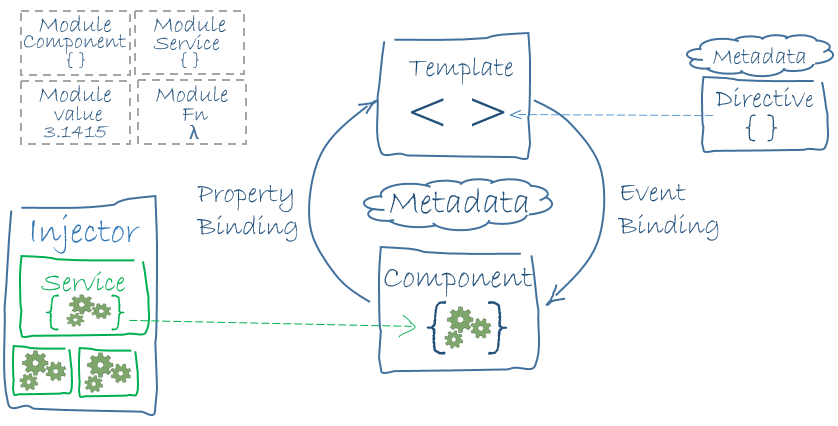
\includegraphics[width=0.8\textwidth]{images/angular}
	\caption{Angular Architektur \cite{MELD.CH3-web-app.angular}}
	\label{fig:angulararch}
\end{figure}



\begin{table}[!htb]
\centering
\resizebox{\columnwidth}{!}{%
\begin{tabular}{ll}
\hline
\multicolumn{2}{|c|}{\textbf{Ember 2.0}}                                                                                                                                                                                                                                            \\ \hline
\multicolumn{1}{|c|}{\textbf{Stärken}}                                                                                                                                    & \multicolumn{1}{c|}{\textbf{Schwächen}}                                                                 \\ \hline
\multicolumn{1}{|l|}{Performance}                                                                                                                                         & \multicolumn{1}{l|}{\begin{tabular}[c]{@{}l@{}}Schwirige Anwendung in speziellen\\ Fällen\end{tabular}} \\ \hline
\multicolumn{1}{|l|}{Rendering am Server}                                                                                                                                 & \multicolumn{1}{l|}{Kleinere Community}                                                                 \\ \hline
\multicolumn{1}{|l|}{Native GUI}                                                                                                                                          & \multicolumn{1}{l|}{}                                                                                   \\ \hline
\multicolumn{1}{|l|}{\begin{tabular}[c]{@{}l@{}}Herangehensweise eines Frameworks \\ (spezifische Funktionen von Angular \\ können einfach entfernt werden)\end{tabular}} & \multicolumn{1}{l|}{}                                                                                   \\ \hline
\multicolumn{1}{|l|}{Dokumentation}                                                                                                                                       & \multicolumn{1}{l|}{}                                                                                   \\ \hline
\multicolumn{1}{|l|}{CLI Tools} & \\ \hline                                                                   
\end{tabular}
}
\caption{Ember 2.0 \url{http://emberjs.com/}}
\end{table}

\textbf{Ember.js 2.0} ähnelt sehr stark dem Angulars Architektur Konzept. Der Grund wieso wir Ember nicht verwenden basiert auf der simplen, etwas schöneren API von Angular. Fakt ist, dass Angular keine weiteren Dependencies hat (Ember.js verwendet jQuery und Handlebars) und dass Angular eine viel geringere Filegröße hat \cite{MELD.CH3-web-app.ember}.

\begin{figure}[!htb]\centering
	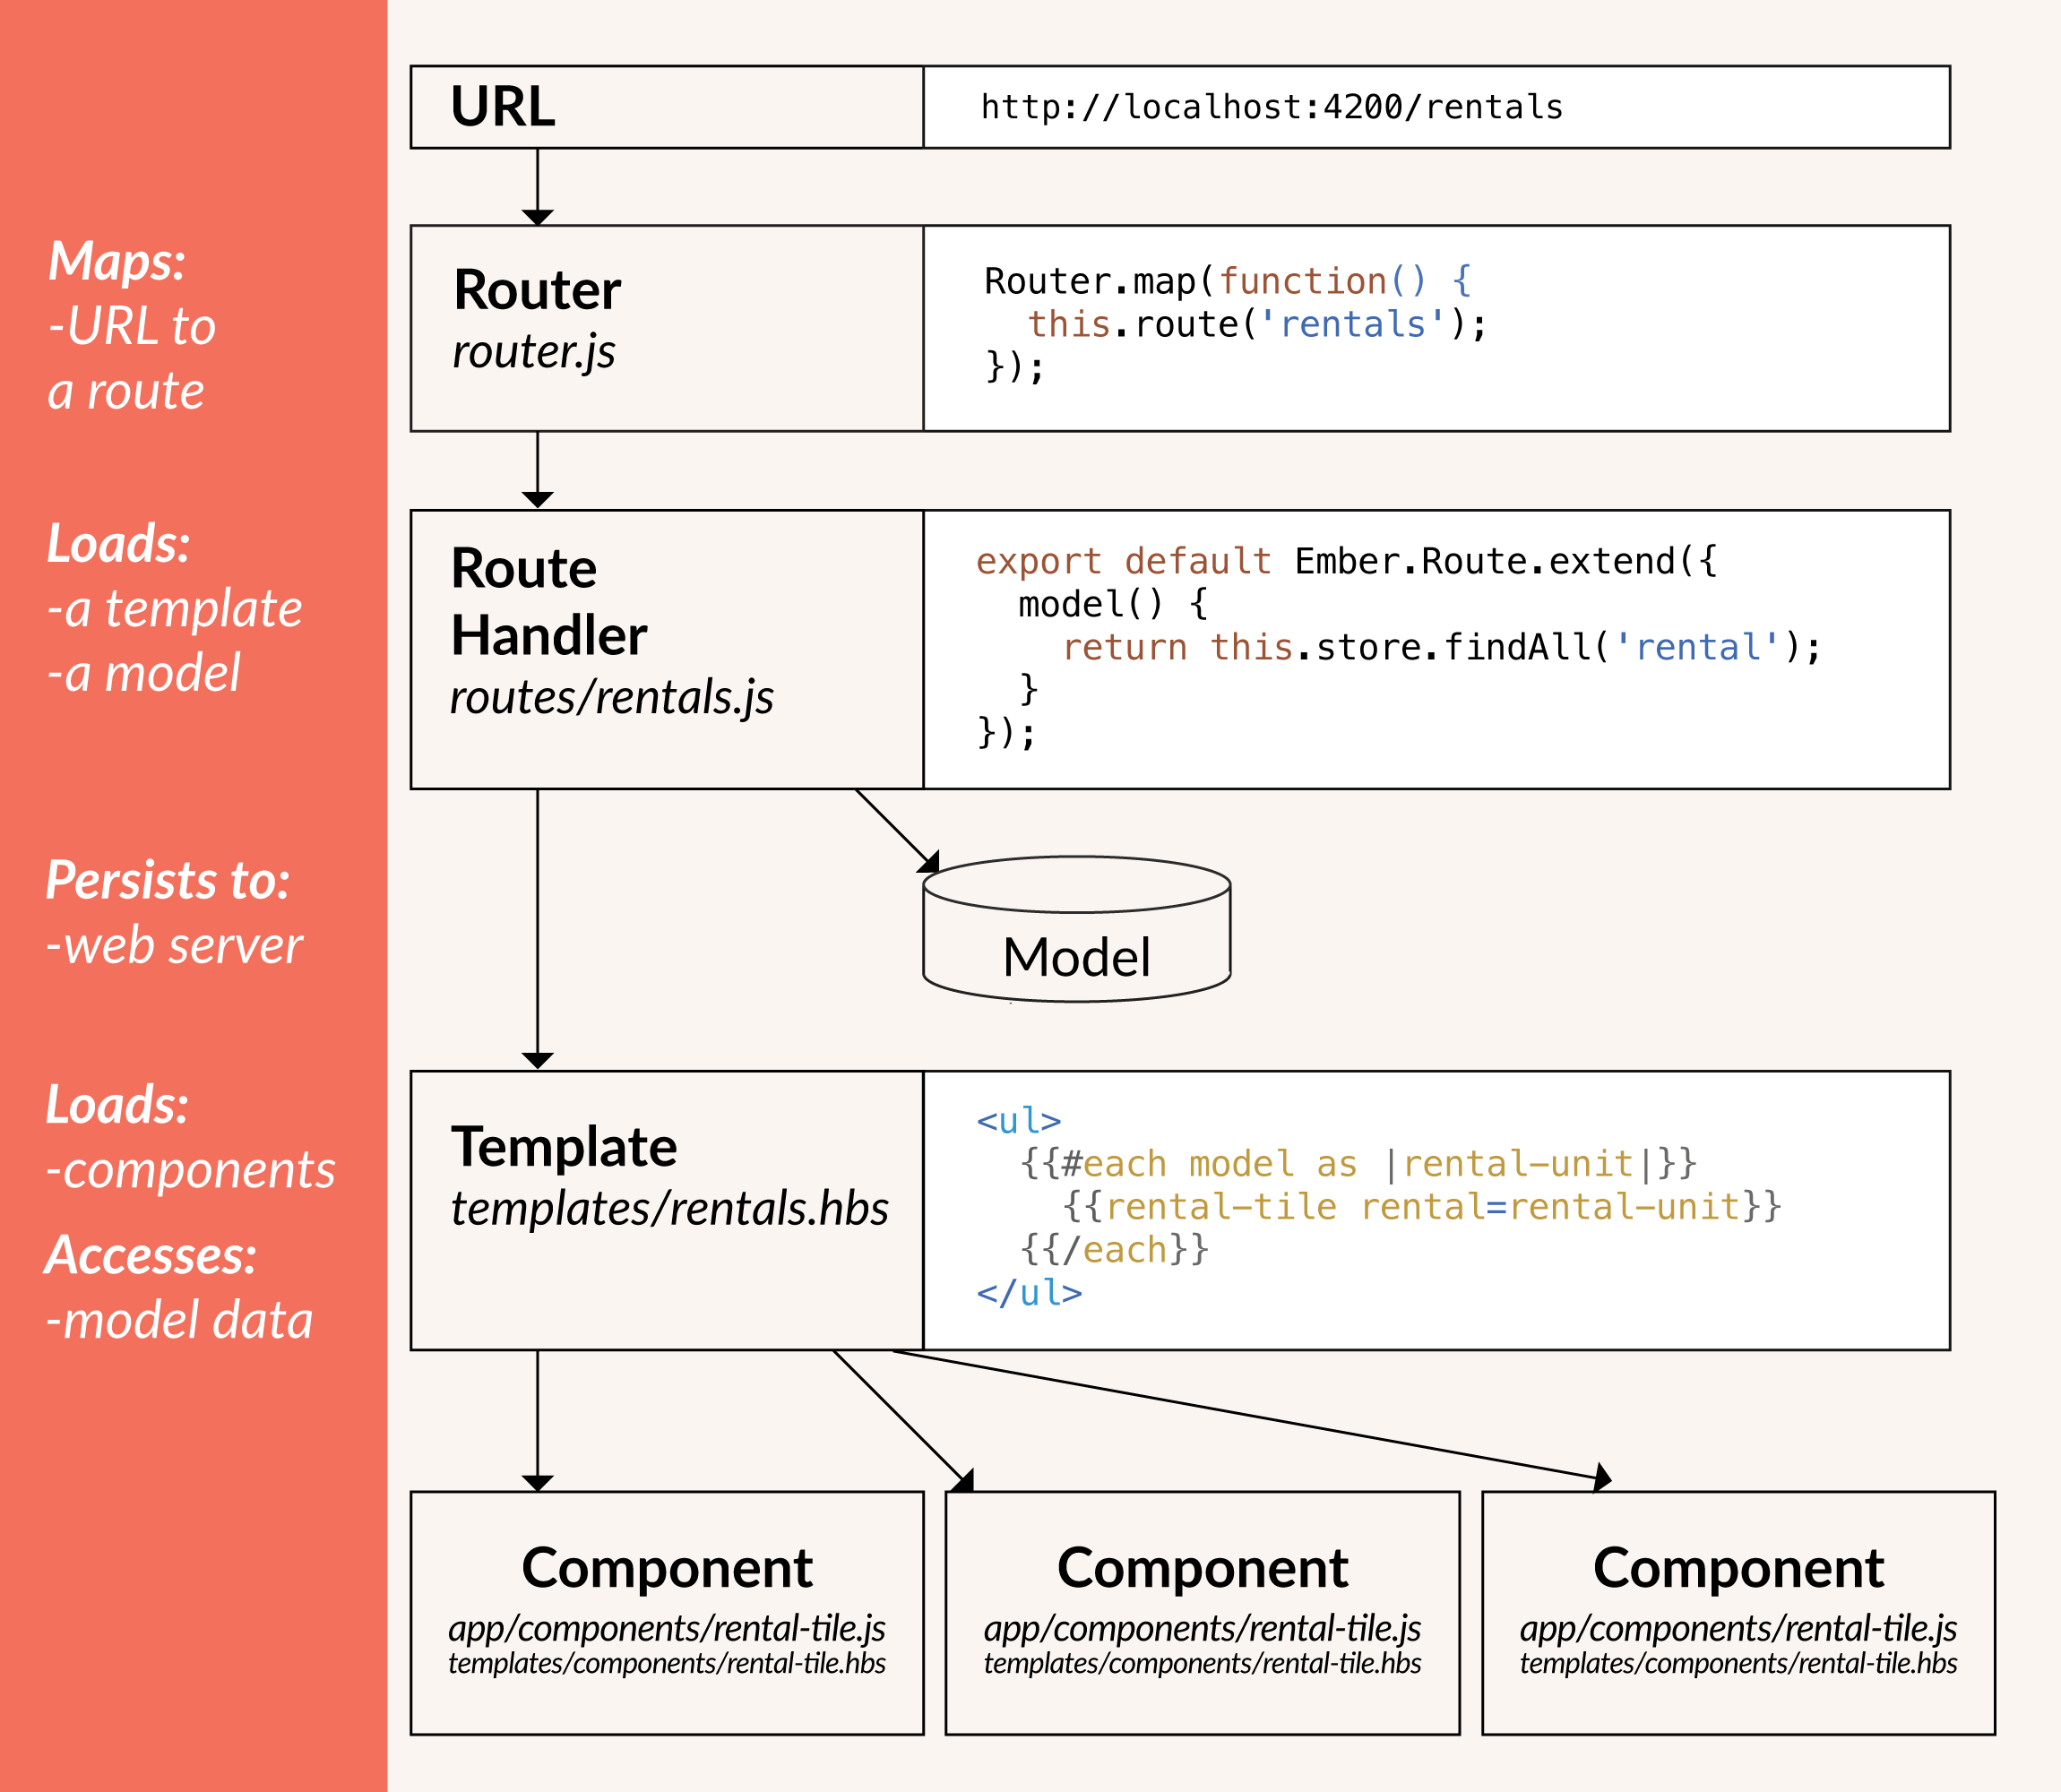
\includegraphics[width=0.6\textwidth]{images/ember}
	\caption{Ember Architektur \cite{MELD.CH3-web-app.ember}}
\end{figure}

\clearpage

\begin{table}[!htb]
\centering
\resizebox{\columnwidth}{!}{%
\begin{tabular}{ll}
\hline
\multicolumn{2}{|c|}{\textbf{React 1.0}}                                                                                                                                                                                                                                                             \\ \hline
\multicolumn{1}{|c|}{\textbf{Stärken}}                                                                                                                                    & \multicolumn{1}{c|}{\textbf{Schwächen}}                                                                                  \\ \hline
\multicolumn{1}{|l|}{Performance}                                                                                                                                         & \multicolumn{1}{l|}{\begin{tabular}[c]{@{}l@{}}Andere Architektur als bei gängigen\\ Frameworks / Libaries\end{tabular}} \\ \hline
\multicolumn{1}{|l|}{Rendering am Server}                                                                                                                                 & \multicolumn{1}{l|}{Unnötig hinzugefügte Features}                                                                       \\ \hline
\multicolumn{1}{|l|}{Native GUI}                                                                                                                                          & \multicolumn{1}{l|}{}                                                                                                    \\ \hline
\multicolumn{1}{|l|}{\begin{tabular}[c]{@{}l@{}}Herangehensweise eines Frameworks \\ (spezifische Funktionen von Angular \\ können einfach entfernt werden)\end{tabular}} & \multicolumn{1}{l|}{}                                                                                                    \\ \hline
\multicolumn{1}{|l|}{Einfach anzuwenden}                                                                                                                                  & \multicolumn{1}{l|}{}                                                                                                    \\ \hline
\multicolumn{1}{|l|}{ES2015 Standard includiert} & \\ \hline                                                                   
\end{tabular}
}
\caption{React 1.0 \url{https://facebook.github.io/react/}}
\end{table}

Das von Facebook entwickelte \textbf{React.js} ist ein eher spezielles Framework, oftmals wird gesagt, dass React.js das \textbf{V} im MVC-Konzept (Model-View-Control) da bietet. Aufgrund dessen ist die Filegröße des Frameworks um einiges kleiner als bei den anderen beiden, bietet aber dennoch viele der Basis Features an \cite{MELD.CH3-web-app.react}. Leider bietet React nicht alles an, was für unsere Applikation benötigt wird, daher ging es rasch aus der ängeren Auswahl raus.

\begin{figure}[!htb]\centering
	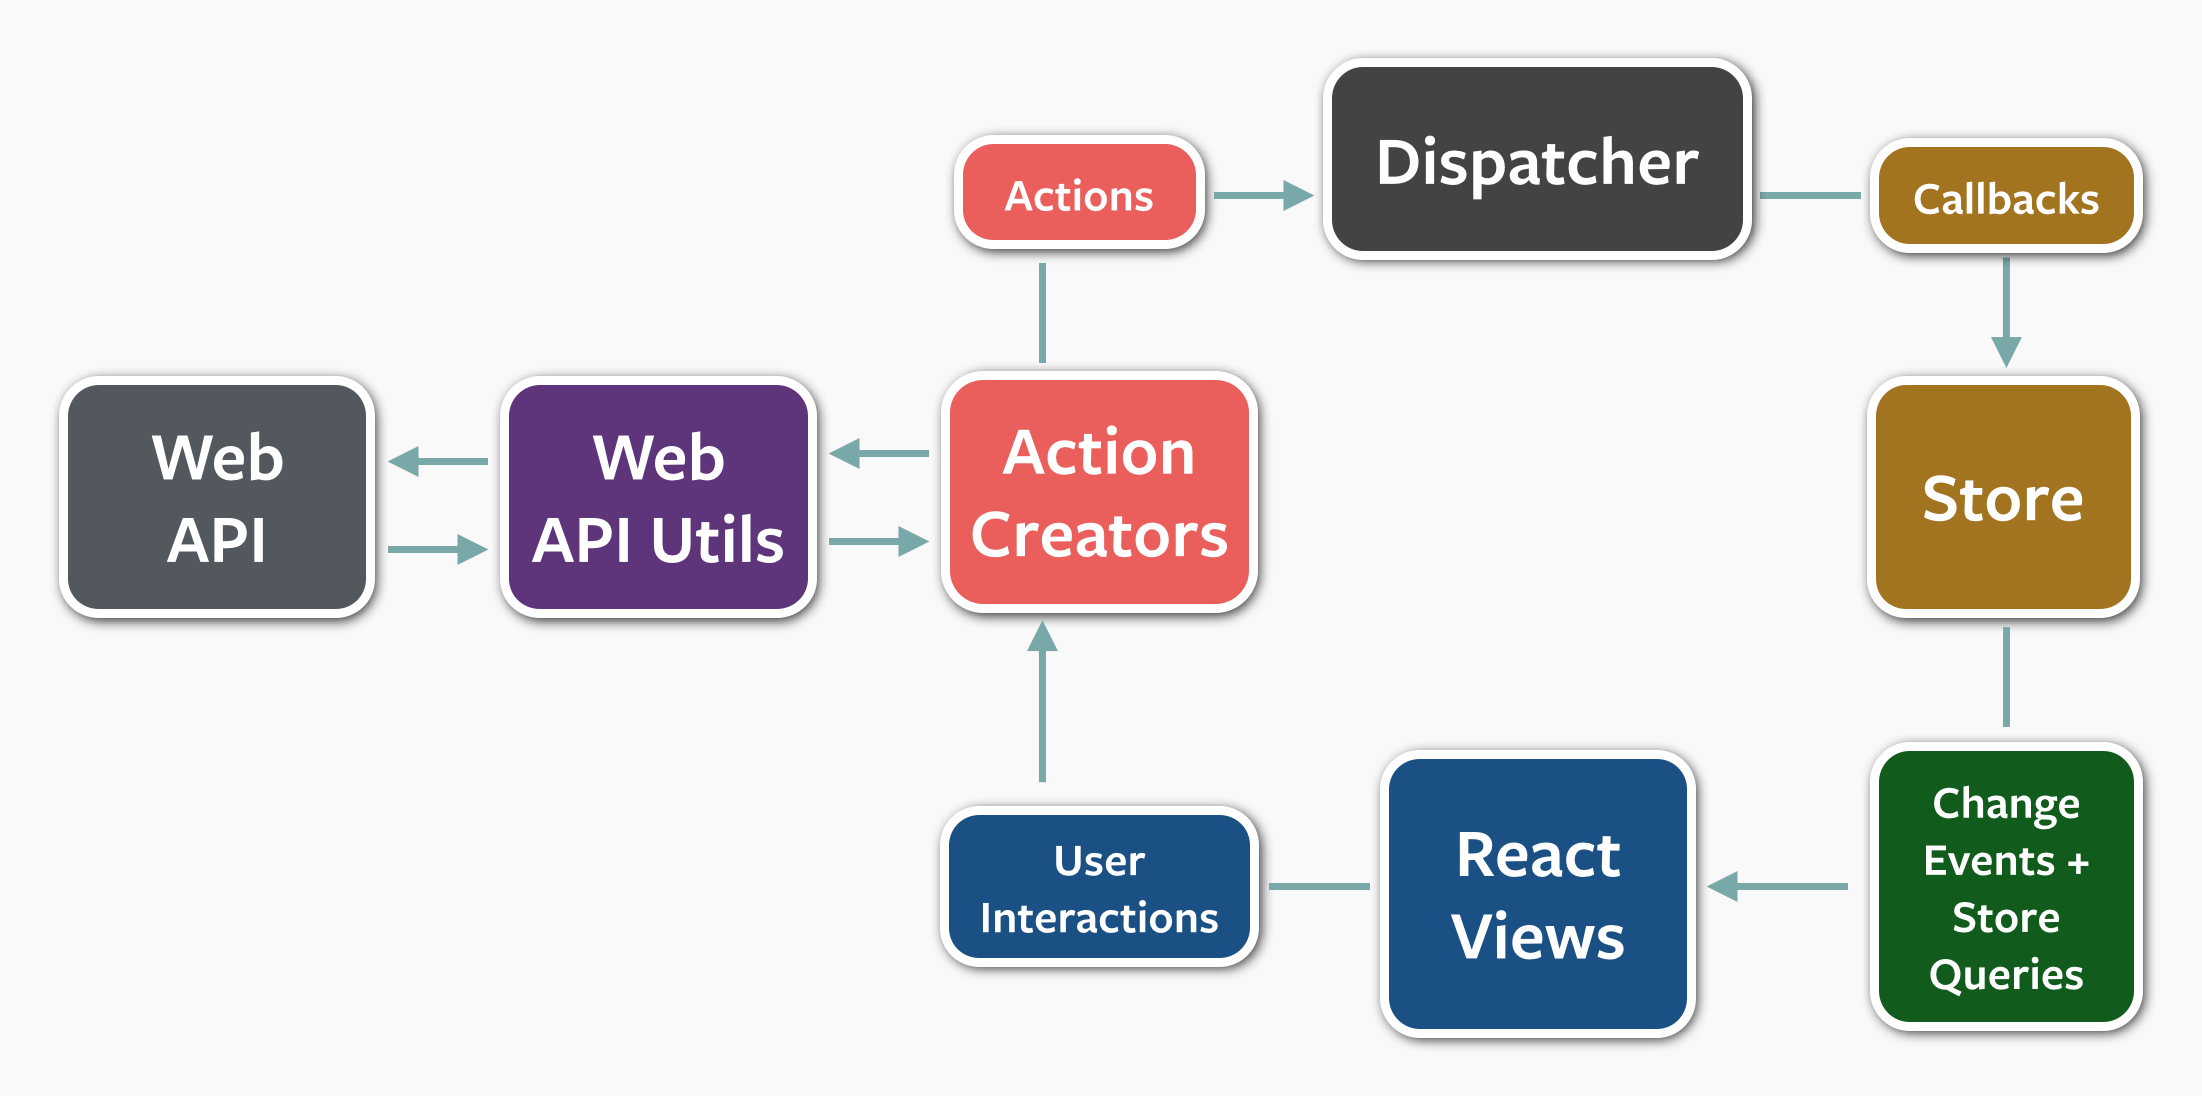
\includegraphics[width=0.8\textwidth]{images/react}
	\caption{React Architektur \cite{MELD.CH3-web-app.react}}
\end{figure}

\clearpage
\subsubsection{Code Standards und Guidelines}
\lfoot{Daniel Melichar}

Für den weiteren Verlauf des Web-App mussten gewisse Standards für den Code gesetzt werden, damit alle auf die selbe Art und Weise programmieren. Das Ziel dieses Style Guides ist, eine Sammlung von Best Practices und Gestaltungsrichtlinien für AngularJS-Anwendungen aufzuzeigen. Sie wurden aus den folgenden Quellen zusammengestellt:

\begin{enumerate}
\def\labelenumi{\arabic{enumi}.}
\item AngularJS Dokumentation
\item Quelltexte oder Artikel
\item Erfahrung des Teams und Lehrer
\end{enumerate}

Für allgemeinen Richtlinien der JavaScript-Entwicklung sollte man folgende Guides begutachten:

\begin{enumerate}
\def\labelenumi{\arabic{enumi}.}
\item \href{http://google-styleguide.googlecode.com/svn/trunk/javascriptguide.xml}{Googles JavaScript-Style-Guide (empfohlen)}
\item \href{https://developer.mozilla.org/en-US/docs/Developer_Guide/Coding_Style}{Mozillas JavaScript-Style-Guide}
\item \href{https://github.com/styleguide/javascript}{GitHubs JavaScript-Style-Guide}
\item \href{http://javascript.crockford.com/code.html}{Douglas Crockfords JavaScript-Style-Guide}
\item \href{https://github.com/airbnb/javascript}{Airbnb JavaScript-Style-Guide}
\end{enumerate}

Automatisierung des Workflows durch: 
\begin{enumerate}
\item Yeoman - \url{http://yeoman.io}
\item Grunt - \url{http://gruntjs.com}
\item Bower - \url{http://bower.io}
\end{enumerate}

\clearpage

\textbf{Verzeichnisstruktur\newline}
Da eine große AngularJS-Anwendung viele Komponenten hat, sollten diese mit Hilfe einer Verzeichnishierarchie strukturiert werden. Auf einer oberen Ebene eine Aufteilung nach Art der Komponenten und auf einer tieferen Ebene eine Aufteilung nach Funktionalität.

Die Verzeichnisstruktur wird in diesem Fall folgendermaßen aussehen:\newline

\dirtree{%
.1 app .
.2 app.js .
.2 controllers .
.3 page1 .
.4 FirstCtrl.js .
.4 SecondCtrl.js .
.3 page2 .
.4 ThirdCtrl.js .
.2 directives .
.3 page1 .
.4 directive1.js .
.3 page2 .
.4 directive2.js .
.4 directive3.js .
.2 filters .
.3 page1 .
.3 page2 .
.2 services .
.3 CommonService.js .
.3 cache .
.4 Cache1.js .
.4 Cache2.js .
.3 models .
.4 Model1.js .
.4 Model2.js .
.1 partials .
.1 lib .
.1 test .
}

\clearpage

\textbf{Markup\newline}
Auch der HTML-Markup ist wichtig und sollte in einem Team so geschrieben werden, als sei sie von derselben Person. Scripts sollten am Ende einer Seite eingefügt werden.

\begin{lstlisting}
<!DOCTYPE html>
<html lang="en">
<head>
  <meta charset="utf-8">
  <title>Meine App</title>
</head>
<body>
  <div ng-app="myApp">
    <div ng-view></div>
  </div>
  <script src="angular.js"></script>
  <script src="app.js"></script>
</body>
</html>
\end{lstlisting}


Um den Code nicht unnötig zu verkomplizieren, fügt man AngularJS-spezifische Direktiven hinter Standard-Attributen ein. Dadurch ist es einfacher, sich den Code anzusehen und durch das Framework erweitertes HTML zu erkennen (was die Wartbarkeit verbessert).

\begin{lstlisting}
<form class="frm" ng-submit="login.authenticate()">
<div>
<input class="ipt" type="text" placeholder="name" require ng-model="user.name">
</div>
</form>
\end{lstlisting}


\textbf{Namensgebung\newline}

\begin{tabular}{|l|l|l|l|}
\hline
\textbf{Element} & \textbf{Style} & \textbf{Beispiel} & \textbf{Verwendung bei} \\ \hline
Module & lowerCamelCase & angularApp &  \\ \hline
Controller & funktionalität + \'Ctrl\' & adminCtrl &  \\ \hline
Direktiven & lowerCamelCase & userInfo &  \\ \hline
Filter & lowerCamelCase & userFilter &  \\ \hline
Services & UpperCamelCase & User & Konstruktor \\ \hline
Services & lowerCamelCase & dataFactory & sonstige \\ \hline
\end{tabular}

\textbf{Module\newline}
Module sollten in lowerCamelCase benannt werden. Um deutlich zu machen, dass das Modul \textit{b} ein Untermodul von \textit{a} ist, kannst man sie durch Namespaces verschachteln, z. B.: \textit{a.b}.

Es gibt zwei verbreitete Wege, nach denen Module strukturiert werden können: Nach Funktionalität
oder nach Typ der Komponente. Derzeit gibt es keinen großen Unterschied, aber die erste Variante sieht sauberer aus. Außerdem wird - wenn lazy-loading für die Module implementiert ist - die Performance der verbessert.

\textbf{Services\newline}
Dieser Abschnitt enthält Informationen über AngularJS' Service-Komponente. Er bezieht sich nicht auf eine spezielle Definitionsweise (d.h. als Provider, Factory oder Service), falls nicht ausdrücklich genannt.

Services in camelCase benennen, bzw UpperCamelCase (PascalCase), um Services zu benennen, die als Konstruktoren verwendet werden, d.h.:

\begin{lstlisting}[language=JavaScript]
module.controller('MainCtrl', function ($scope, User) {
  $scope.user = new User('foo', 42);
});

module.factory('User', function () {
  return function User(name, age) {
    this.name = name;
    this.age = age;
  };
});
\end{lstlisting}

Alle anderen Service in lowerCamelCase benennen. Kapsle die gesamte Anwendungslogik in Services.Services, die eine bestimmte Domäne abbilden, sollten bevorzugt als \textit{service} statt als \textit{factory} geschrieben werden. Auf diese Weise können die Vorteile der klassischen Vererbung einfacher genutzt werden:

\begin{lstlisting}[language=JavaScript]
function Human() {
  // body
}
Human.prototype.talk = function() {
  return "I'm talking";
};

function Developer() {
  // body
}
Developer.prototype = Object.create(Human.prototype);
Developer.prototype.code = function() {
  return "I'm coding";
};

myModule.service('Human', Human);
myModule.service('Developer', Developer);
\end{lstlisting}

Für einen sitzungsbezogenen Cache kannst du \textit{\$cacheFactory} verwenden. Diesen sollte man nutzen, um die Ergebnisse von Anfragen oder aufwändigen Berechnungen zwischenzuspeichern.Falls ein Service konfiguriert werden muss, definirt man ihn als Provider und konfiguriert im \textit{config}-Callback, wie hier:

\begin{lstlisting}[language=JavaScript]
angular.module('demo', [])
.config(function ($provide) {
  $provide.provider('sample', function () {
    var foo = 42;
    return {
      setFoo: function (f) {
        foo = f;
      },
      $get: function () {
        return {
          foo: foo
        };
      }
    };
  });
});

var demo = angular.module('demo');

demo.config(function (sampleProvider) {
  sampleProvider.setFoo(41);
});
\end{lstlisting}

\clearpage
\subsubsection{Prototypische Implementierung}

Lorem ipsum dolor sit amet, consectetur adipisicing elit, sed do eiusmod
tempor incididunt ut labore et dolore magna aliqua. Ut enim ad minim veniam,
quis nostrud exercitation ullamco laboris nisi ut aliquip ex ea commodo
consequat. Duis aute irure dolor in reprehenderit in voluptate velit esse
cillum dolore eu fugiat nulla pariatur. Excepteur sint occaecat cupidatat non
proident, sunt in culpa qui officia deserunt mollit anim id est laborum.

\clearpage

\clearpage % DO NOT REMOVE